%%
%% Copyright 2007, 2008, 2009 Elsevier Ltd
%%
%% This file is part of the 'Elsarticle Bundle'.
%% ---------------------------------------------
%%
%% It may be distributed under the conditions of the LaTeX Project Public
%% License, either version 1.2 of this license or (at your option) any
%% later version.  The latest version of this license is in
%%    http://www.latex-project.org/lppl.txt
%% and version 1.2 or later is part of all distributions of LaTeX
%% version 1999/12/01 or later.
%%
%% The list of all files belonging to the 'Elsarticle Bundle' is
%% given in the file `manifest.txt'.
%%

%% Template article for Elsevier's document class `elsarticle'
%% with numbered style bibliographic references
%% SP 2008/03/01
%%
%%
%%
%% $Id: elsarticle-template-num.tex 4 2009-10-24 08:22:58Z rishi $
%%
%%
\documentclass[preprint,12pt,3p]{elsarticle}

%% Use the option review to obtain double line spacing
%% \documentclass[preprint,review,12pt]{elsarticle}

%% Use the options 1p,twocolumn; 3p; 3p,twocolumn; 5p; or 5p,twocolumn
%% for a journal layout:
%% \documentclass[final,1p,times]{elsarticle}
%% \documentclass[final,1p,times,twocolumn]{elsarticle}
%% \documentclass[final,3p,times]{elsarticle}
%% \documentclass[final,3p,times,twocolumn]{elsarticle}
%% \documentclass[final,5p,times]{elsarticle}
%% \documentclass[final,5p,times,twocolumn]{elsarticle}

%% if you use PostScript figures in your article
%% use the graphics package for simple commands
%% \usepackage{graphics}
%% or use the graphicx package for more complicated commands
%% \usepackage{graphicx}
%% or use the epsfig package if you prefer to use the old commands
%% \usepackage{epsfig}

%% The amssymb package provides various useful mathematical symbols
\usepackage{amssymb}
%% The amsthm package provides extended theorem environments
%% \usepackage{amsthm}

%% The lineno packages adds line numbers. Start line numbering with
%% \begin{linenumbers}, end it with \end{linenumbers}. Or switch it on
%% for the whole article with \linenumbers after \end{frontmatter}.
%% \usepackage{lineno}

%% natbib.sty is loaded by default. However, natbib options can be
%% provided with \biboptions{...} command. Following options are
%% valid:

%%   round  -  round parentheses are used (default)
%%   square -  square brackets are used   [option]
%%   curly  -  curly braces are used      {option}
%%   angle  -  angle brackets are used    <option>
%%   semicolon  -  multiple citations separated by semi-colon
%%   colon  - same as semicolon, an earlier confusion
%%   comma  -  separated by comma
%%   numbers-  selects numerical citations
%%   super  -  numerical citations as superscripts
%%   sort   -  sorts multiple citations according to order in ref. list
%%   sort&compress   -  like sort, but also compresses numerical citations
%%   compress - compresses without sorting
%%
%% \biboptions{comma,round}

% \biboptions{}


\journal{Neural Networks}

\begin{document}

\begin{frontmatter}

\title{Sample article to present \texttt{elsarticle} class\tnoteref{label0}}
\tnotetext[label0]{This is only an example}


\author[label1,label2]{Author One\corref{cor1}\fnref{label3}}
\address[label1]{Address One}
\address[label2]{Address Two\fnref{label4}}

\cortext[cor1]{I am corresponding author}
\fntext[label3]{I also want to inform about\ldots}
\fntext[label4]{Small city}

\ead{author.one@mail.com}
\ead[url]{author-one-homepage.com}

\author[label5]{Author Two}
\address[label5]{Some University}
\ead{author.two@mail.com}

\author[label1,label5]{Author Three}
\ead{author.three@mail.com}

\begin{abstract}
Text of abstract. Text of abstract. Text of abstract. Text of abstract. Text of abstract. 
\end{abstract}

\begin{keyword}
%% keywords here, in the form: keyword \sep keyword
foraging \sep active learning \sep template
%% MSC codes here, in the form: \MSC code \sep code
 or \MSC[2008] code \sep code (2000 is the default)
\end{keyword}

\end{frontmatter}

%%
%% Start line numbering here if you want
%%
% \linenumbers


	%\section{BACKGROUND}
\label{sec:background}

%\cite{thompson2008intelligent} work in the Atacama desert was about geologic survey and the construction of scientific maps.  The strategy relied on prior knowledge in the form of satellite imagery.  Further the work did not correlate the remote sensing with a secondary, hidden parameter, as is the case for characterising sub-surface habitats.  From \cite{smith2008xxx} employed a POMDP appraoch to address this problem, finding trajectories that maximize the probability of finding life, however their things do not scale to planetary scale.  

%The approach used in multi-armed bandit models scale more effectively than
%POMDPs.  Multi-armed bandits is a formulation for the sequential selection of
%experiments which models the different possible experiments as arms of a slot
%machine, with each arm.  
Previous approaches to planetary scale science autonomy fall down in two
respects.  Firstly, these approaches model scientific exploration as a standard
exploration/exploitation problem.  A model that does not necessarily hold for
planetary exploration.  Secondly, they do not use the output of the scientific
measurements to improve how the robots select between sampling actions.  For
stationary processes experiment design dictates that the optimal set
of experiments can be determined without ever knowing the results of those
experiments \cite{srinivas2009gaussian}.

\subsection{Sequential Action Selection}

Sequential experiment selection, a type of active learning, is addressed in the
multi-armed bandit literature.  The multi-armed bandit was introduced in
\cite{robbins1952some} as a means of sequentially selecting which experiments
to conduct with a limited budget.  In Robbins' work \cite{robbins1952some}
selecting experiments is modelled on determining the
payouts of one-armed bandit machines -- each machine represents a different
experiment.  The player has a fixed sampling budget and has to sequentially
choose which machine to play, trading off exploiting the expected rewards for
the different arms and exploring the different arms learning more accurately
the payouts of those arms.  

Lai \emph{et al.} \cite{lai1985asymptotically} introduced the Upper Confidence
Bound (UCB) rule which values sampling opportunities with the sum of the expected reward for a sampling opportunity and a term that tries to balance the samples amongst all types of sampling opportunities.

$$
Value = \mathbb{E}\left[R_i\right] + \sqrt{\frac{2\ln t_i}{T}}
$$

Where $R_i$ is the reward for sampling opportunity $i$, $t_i$ is the number of times $i$ has been sampled, and $T$ is the total number of samples distributed.  Work on proving the bounds of this algorithm has been continued by Agarawal \cite{agrawal1995sample} and Auer and Ortner\cite{auer2010ucb}.  

%  In the UCB algorithm the measure of
%informativeness is the standard error of the reward function, a value that
%decreases not only with the number of samples taken but also with the
%variability of the reward distribution. 
%\cite{agrawal1995sample} and \cite{auer2010ucb} continue
%work on UCB algorithms and introduce a metric that
%combines reward and a measure of how infrequently a given arm has been sampled
%relative to the total samples spent.

Other approaches to the bandit problem use reward plus the uncertainty of that
reward to indicate value.  We see this in the work of Burnetas and Katehakis
\cite{burnetas1997optimal} and Auer \cite{auer2003using}.  This is a sentiment
seen in other work, like the optimistic planners of Jurgen Schmidhuber's group
\cite{schmidhuber1997what,schmidhuber2003exploring,schmidhuber2009simple,sun2011planning}.
They choose actions that maximize the expected information gain with respect to
some model they are learning.  The most valuable actions are the ones that
result in the greatest shift in the distribution the learner is building.

Balcan \cite{balcan2006agnostic} presents a method for learning classifiers by
requesting samples from the input space with the greatest classification
error.  Classification error and uncertainty in function value
are fungible quantities in this case.  An analogy can be drawn between
the classifiers used in \cite{balcan2006agnostic} and the bandit arms used by
Auer and Ortner\cite{auer2010ucb}.

Thompson and Wettergreen \cite{thompson2008intelligent} maximize diversity of
collected samples by using mutual information sampling.  This approach ensures
diversity in the collected sample set, an act that reduces uncertainty in the
input space of a function.  Neither mutual information nor maximum entropy
sampling methods, when used with stationary Gaussian processes, take into
account the dependent variable when selecting samples.  

Sequential experiment selection values actions by a combination of reward and
uncertainty in that reward.  Since the mission of exploration is learning the
reward is the reduction in uncertainty by taking actions.  Seeking uncertainty
is a useful way to value options presented to a learning agent but it does not
address the explorer's problem of either giving up on a sampling opportunity
or searching for better opportunities.  Further it is not guaranteed that
sampling opportunities can be accessed at no cost, an assumption commonly made
when querying an oracle.


\subsection{Exploration as Foraging}

% The exploration/exploitation problem asks the question: Is an agent rewarded
% better by exploiting already acquired knowledge or by exploring different
% options and improving that knowledge?  The multi-armed bandit
% \cite{robbins1952some} was introduced to address the exploration/exploitation
% trade-off with a limited sampling budget.  Multi-armed bandits model a fixed
% list of experiments as different slot machines each with their own random
% payout.  An arm of a bandit is a metaphor for a random variable and
% the reward for playing that arm reveals information about that random variable.
% A shortcoming of the multi-armed bandit approach is that it assumes that at any
% given time all random variables are known and are available to conduct.  


Active learning assumes an oracle and as such does not map well to exploration
in unknown environments.  In approaches like those of Robbins
\cite{robbins1952some} or Balcan \cite{balcan2006agnostic} the agent conducting
experiments has at any time the opportunity to sample random variable they
are characterizing.  This is not the case in planetary exploration, we can only
sample from those random variables that are present as robots follow their
trajectories.  The inaccuracy of the oracle model has been previously identified by Donmez and Carbonell \cite{donmez2008proactive}.

Foraging theory provides a way to make the decision to stay or to go
 withouth knowledge of future opportunities.  This stands in contrast to the
standard exploration/exploitation problem choosing from known sampling
opportunities.

% To help the robot scientist make the decision to leave or not we employ a model
% of optimal foraging based on Mean Value Theorem
% \cite{kolling2012neural},\cite{charnov1976optimal} to choose between available
% opportunities and unknown future opportunities.  


Optimal foraging strategies devised by Charnov \cite{charnov1976optimal}
describe how predators hunt in different geographic regions with different
levels of resources.  Animals make the decision to forage by comparing the
value of the options it has in front of it to the expected value of what it may
obtain by searching for better options \cite{kolling2012neural}, less the cost
of conducting a search.  

Kolling \emph{et al} \cite{kolling2012neural} found that humans make foraging
decisions based on the arithmetic mean of the estimated values of the options
they are presented with and the options that remain in the surrounding
environment.  From foraging literature we learn to compute the value of
searching in an environment by taking the arithmetic mean of what is thought to
be in that environment.  The decision rule to stay or leave is a comparison
between the value of the current opportunity and the expected value of the
environment.

Optimal foragers considering three things when choosing to leave a resource:
Expected value of the current opportunity, the expected value of the rest of
the environment, and the cost of searching for new opportunities
\cite{charnov1976optimal},\cite{kolling2012neural}.  To adapt foraging to
exploration we need to answer the question: What is the value of
an option presented to the explorer?  To answer that question we look to active
learning.

Previous work by the authors \cite{furlong2014sequential} addressed the problem of exploring along a transect by employing techniques from Foraging Theory. However that work did not address the fact that the sampler had a limited budget.  Agents in that work did not expend all of their samples for large budgets, a problem this research addresses.

The strategy presented by Ferri \emph{et al.} made a comparison between the
perceived value of the available sampling opportunity and an arbitrary function
of the remaining number of sampling opportunities \cite{ferri2010novel}.  The
value of a sampling opportunity was determined by a fixed threshold and the
proclivity for spending samples was likewise determined by an arbitrary
constant.  In contrast this work employs an information theoretic measure of opportunity value and a principled measure to determine when to expend a sample. 

% The distinction between exploration/exploitation and forage/engage is
% determined by two things: the recognition that there is not always a choice of
% what to explore and the realisation that the choice is between what is
% available and what may yet be encountered.  


The prior work yields two observations.  Firstly, foraging, a better model for
planetary exploration, requires a measure of value of the sampling
opportunities available to the exploring agent.  Secondly, active learning uses
uncertainty -- in both input and output space of a function -- to value
potential exploration opportunities.  What follows next is a method for
exploring that reflects the limitations of a planetary setting and incorporates
the result of sampling operations into decision making processes.

	%\section{BACKGROUND}
\label{sec:background}

%\cite{thompson2008intelligent} work in the Atacama desert was about geologic survey and the construction of scientific maps.  The strategy relied on prior knowledge in the form of satellite imagery.  Further the work did not correlate the remote sensing with a secondary, hidden parameter, as is the case for characterising sub-surface habitats.  From \cite{smith2008xxx} employed a POMDP appraoch to address this problem, finding trajectories that maximize the probability of finding life, however their things do not scale to planetary scale.  

%The approach used in multi-armed bandit models scale more effectively than
%POMDPs.  Multi-armed bandits is a formulation for the sequential selection of
%experiments which models the different possible experiments as arms of a slot
%machine, with each arm.  
Previous approaches to planetary scale science autonomy fall down in two
respects.  Firstly, these approaches model scientific exploration as a standard
exploration/exploitation problem.  A model that does not necessarily hold for
planetary exploration.  Secondly, they do not use the output of the scientific
measurements to improve how the robots select between sampling actions.  For
stationary processes Bayesian experiment design dictates that the optimal set
of experiments can be determined without ever knowing the results of those
experiments \cite{srinivas2009gaussian}.  However real world quantities are not
necessarily stationarity and they may not even obey a function.

\subsection{Foraging as Exploration}

The exploration/exploitation problem asks the question: Is an agent rewarded
better by exploiting already acquired knowledge or by exploring different
options and improving that knowledge?  The multi-armed bandit
\cite{robbins1952some} was introduced to address the exploration/exploitation
trade-off with a limited sampling budget.  Multi-armed bandits model a fixed
list of experiments as different slot machines each with their own random
payout.  An arm of a bandit is a metaphor for a random variable and
the reward for playing that arm reveals information about that random variable.
A shortcoming of the multi-armed bandit approach is that it assumes that at any
given time all random variables are known and are available to conduct.  

% The exploration/exploitation problem is about deciding if it is more
% informative to try different machines to learn about their expected payoffs or
% if it is best to continue to play the machine that is currently considered the
% most rewarding.  


Active learning assumes an oracle and as such does not map well to exploration
in unknown environments.  In approaches like those of Robbins
\cite{robbins1952some} or Balcan \cite{balcan2006agnostic} the agent conducting
experiments has at any time the opportunity to sample random variable they
are characterizing.  This is not the case in planetary exploration, we can only
sample from those random variables that are present as robots follow their
trajectories.  The inaccuracy of the oracle model has been previously identified by Donmez and Carbonell \cite{donmez2008proactive}.

Foraging theory provides an answer to the question of whether to stay or to go
 in the face of unknown future opportunities.  This stands in contrast to the
standard exploration/exploitation problem choosing from known sampling
opportunities.

Optimal foraging strategies devised by Charnov \cite{charnov1976optimal}
describe how predators hunt in different geographic regions with different
levels of resources.  Animals make the decision to forage by comparing the
value of the options it has in front of it to the expected value of what it may
obtain by searching for better options \cite{kolling2012neural}, less the cost
of conducting a search.  The distinction between exploration/exploitation and
forage/engage is determined by two things: the recognition that there is not
always a choice of what to explore and the realisation that the choice is
between what is available and what may yet be encountered.  

Kolling \emph{et al} \cite{kolling2012neural} found that humans make foraging
decisions based on the arithmetic mean of the estimated values of the
options they are presented with and the options that remain in the surrounding
environment.  From foraging literature we learn to compute the value of
searching in an environment by taking the arithmetic mean of what is thought to
be in that environment.  The decision rule to stay or leave is a very simple
comparison between the value of the current opportunity and the value of the
environment.

Optimal foragers considering three things when choosing to leave a resource:
Expected value of the current opportunity, the expected value of the rest of
the environment, and the cost of searching for new opportunities
\cite{charnov1976optimal},\cite{kolling2012neural}.  To adapt foraging to
exploration we need to answer the question: What is the value of
an option presented to the explorer?  To answer that question we look to active
learning.

\subsection{Active learning}

In active learning agents get to choose examples in order to resolve
uncertainty or inaccuracy in models they are learning.  An early version of
active learning is the multi-armed bandit problem.  The k-armed bandit was
introduced in \cite{robbins1952some} as a means of sequentially selecting which
experiments to conduct.  In Robbins' work \cite{robbins1952some} selecting which
experiment to conduct next is modelled on determining the payouts of one-armed
bandit machines, where each machine represents a different experiment.  The
player has a fixed sampling budget and has to sequentially choose which machine
to play, trading off exploiting the expected rewards for the different arms and
exploring the different arms learning more accurately the payouts of those
arms.  

Lai \emph{et al.} \cite{lai1985asymptotically} introduced the Upper Confidence
Bound (UCB) rule which values sampling opportunities with the sum of the expected reward for a sampling opportunity and a term that tries to balance the samples amongst all types of sampling opportunities.

$$
Value = \mathbb{E}\left[R_i\right] + \sqrt{\frac{2\ln t_i}{T}}
$$

Where $R_i$ is the reward for sampling opportunity $i$, $t_i$ is the number of times $i$ has been sampled, and $T$ is the total number of samples distributed.  Work on proving the bounds of this algorithm has been continued by Agarawal \cite{agrawal1995sample} and Auer and Ortner\cite{auer2010ucb}.  

%  In the UCB algorithm the measure of
%informativeness is the standard error of the reward function, a value that
%decreases not only with the number of samples taken but also with the
%variability of the reward distribution. 
%\cite{agrawal1995sample} and \cite{auer2010ucb} continue
%work on UCB algorithms and introduce a metric that
%combines reward and a measure of how infrequently a given arm has been sampled
%relative to the total samples spent.

Other approaches to the bandit problem use reward plus the uncertainty of that
reward to indicate value.  We see this in the work of Burnetas and Katehakis
\cite{burnetas1997optimal}, and Auer \cite{auer2003using}.  This is a sentiment
seen in other work, like the optimistic planners of Jurgen Schmidhuber's group
\cite{schmidhuber1997what,schmidhuber2003exploring,schmidhuber2009simple,sun2011planning}.
They choose actions that maximize the expected information gain with respect to
some model they are learning.  The most valuable actions are the ones that
result in the greatest shift in the distribution the learner is building.

Balcan \cite{balcan2006agnostic} presents a method for learning classifiers by
requesting samples in the input space of the function where the classification
error is the greatest.  Classification error and uncertainty in function value
are fungible quantities in this case.  An analogy can be drawn between
the classifiers used in \cite{balcan2006agnostic} and the bandit arms used by
Auer and Ortner\cite{auer2010ucb}.

Thompson and Wettergreen \cite{thompson2008intelligent} maximize diversity of
collected samples by using mutual information sampling.  This approach ensures
diversity in the collected sample set, an act that reduces uncertainty in the
input space of a function.  Neither mutual information nor maximum entropy
sampling methods, when used with stationary Gaussian processes, take into
account the dependent variable when selecting samples.  

The prior work described above assumes one is choosing among a number of
options and want to choose the maximally informative one.  While choosing the
maximally informative option is a useful guiding principle when robot explorers
are presented with a number of sampling opportunities, it does not address the
problem that explorers may have to give up a sampling opportunity in the hopes
of finding better ones.  Further it is not guaranteed that there is no cost
associated with getting to sampling opportunities, an assumption commonly made when querying an oracle.

The prior work yields two observations.  Firstly, foraging, a better model for
planetary exploration, requires a measure of value of the sampling
opportunities available to the exploring agent.  Secondly, active learning uses
uncertainty -- in both input and output space of a function -- to value potential exploration opportunities.  What follows next is a method
for exploring that reflects the limitations of a planetary setting and
incorporates the result of sampling operations into decision making processes.


\section{Method}
\label{sec:method}

The decision making agents in this paper are tested on several randomly
generated transects.  They are repeatedly presented with an object to sample
and have to make the choice to either take a sample or continue travelling
along the transect.  Like the Robbins' secretary problem the agents are not
permitted to backtrack to avail of a previous opportunity.


Figure \ref{fig:transect} gives an example of a simulated transect. As we can
see there are sampling opportunities of different types scattered along the
path that the robot travels along.  

\begin{figure}[htpd!]
	\centering 
	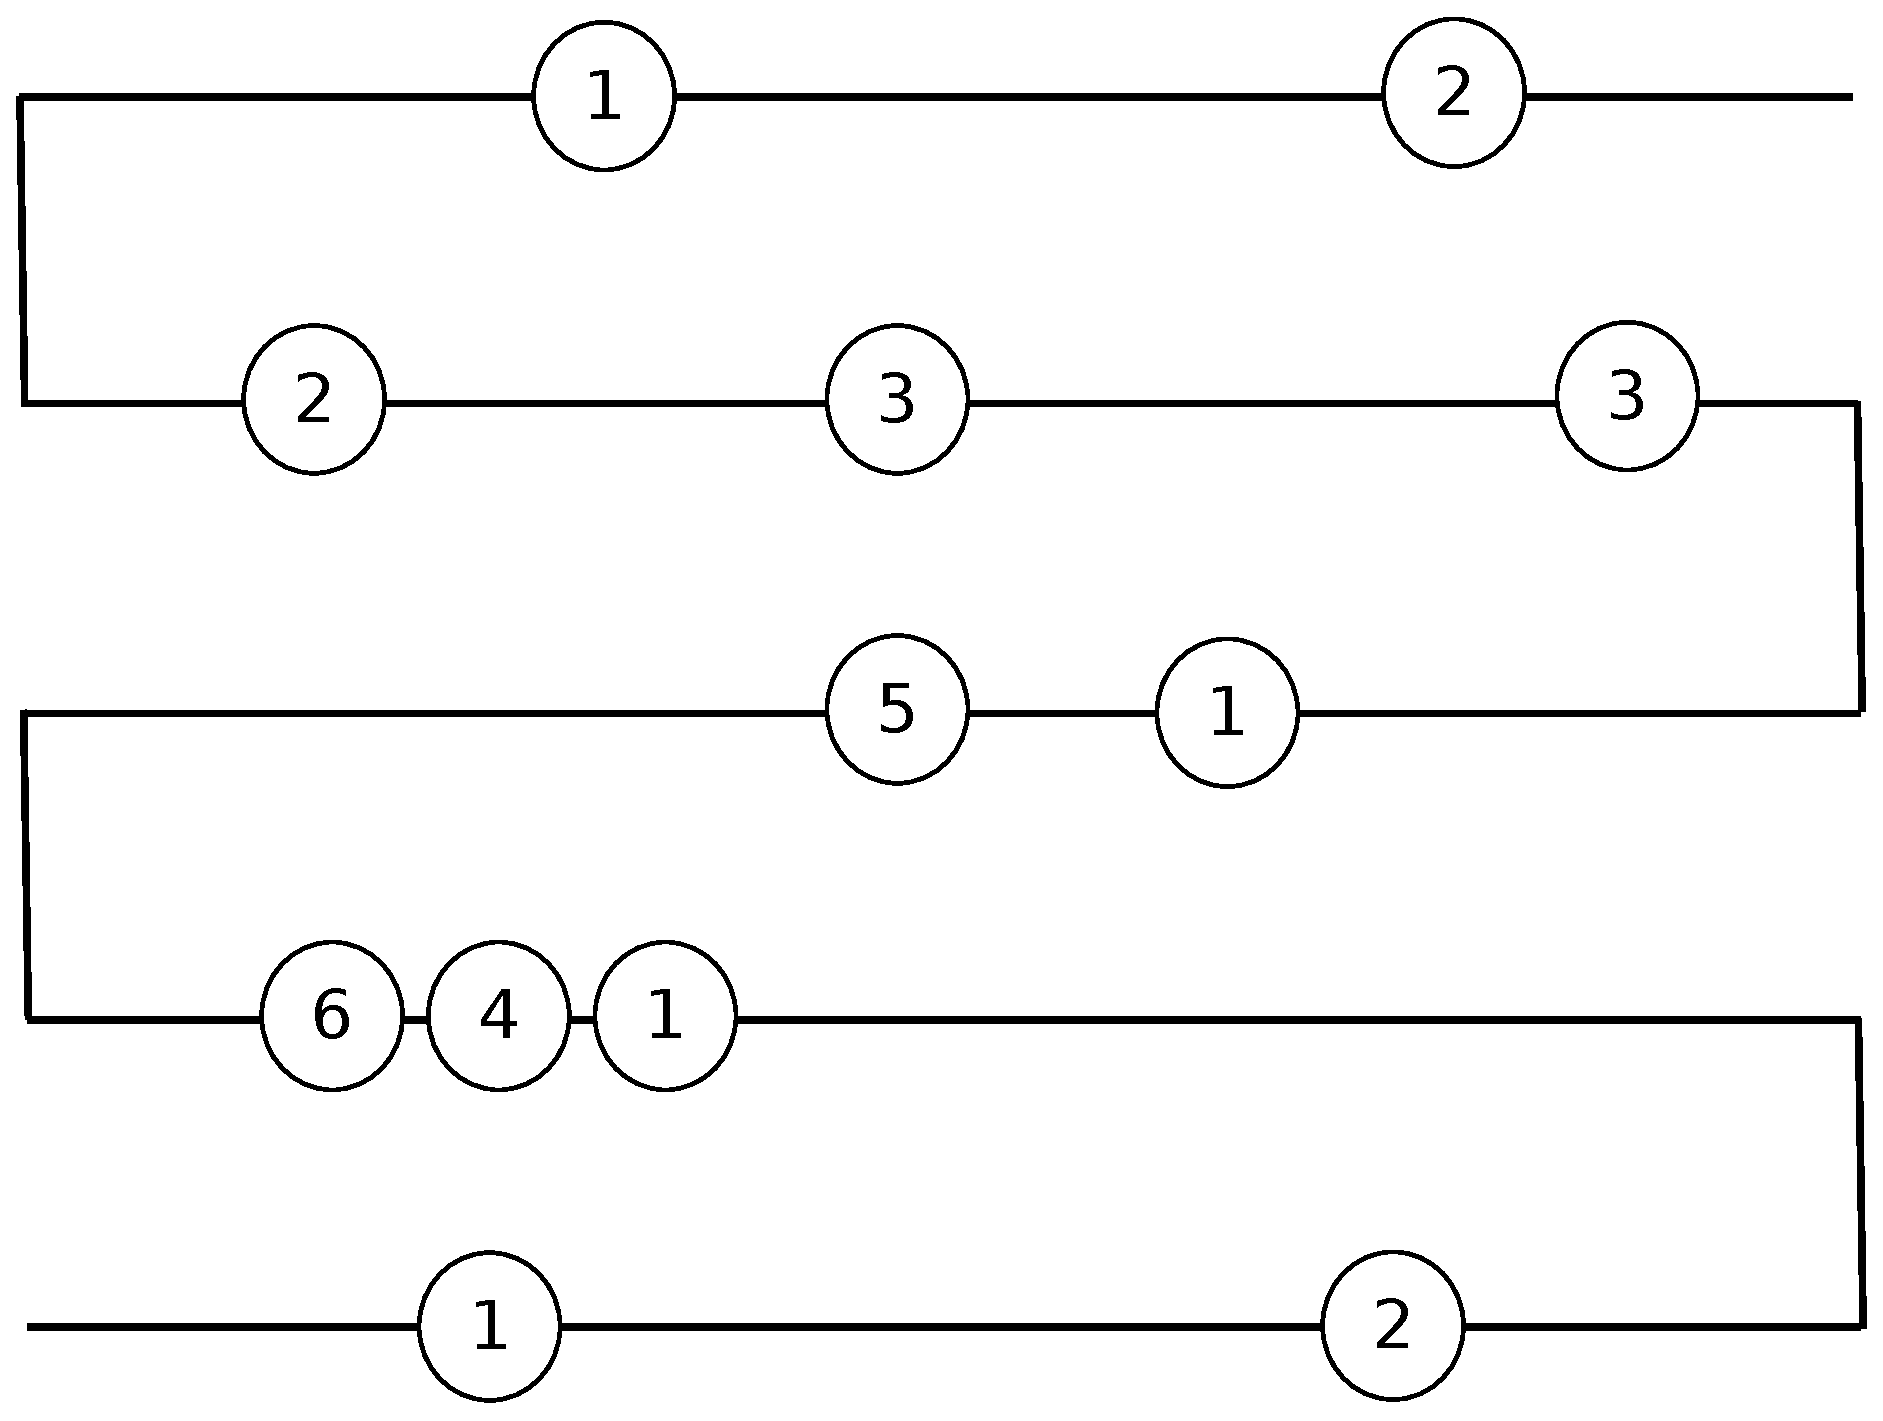
\includegraphics[width=0.8\textwidth]{transect}
	\caption{A cartoon illustrating a transect a robot might be encountering and how samping opportunities of different types may be distributed along it.  In the field the robot would start at one end of the path and follow it to the other end.  There is one path that the rover may follow across the terrain resulting in it encountering different types of sampling opportunities.}
	\label{fig:transect}
\end{figure}


The primary objective of the robot is to learn distributions behind different
classes of objects.  For example they may be the probability distribution
governing the density of sub surface microbial life in different classes of
soil.  Previous work have identified that texture information can successfully
classify different types of soil material \cite{dunlop2006automatic}.  
We imagine that the classes of objects in
this research could correspond to those soil classes.


\subsection{Experiment}

The experiment presented in this paper is a modification of the experiments
presented in \cite{furlong2014sequential} and \cite{furlong2014budgeting}.  In
the prior work agents were equipped with limited sampling budgets.  In this
experiment the agents have an unlimited capacity to take samples, but the time
to take the sample is non-zero and there is an overall limit on the duration of
the mission.  The sampling cost and the overall mission time is given in units of arbitrary time.

As with the previous experiments the agents are not permitted to back track in
the hopes of getting a better opportunity.  The primary reason is to constantly
drive the robot to the end of its exploration mission.  Coverage is an
important part of exploration and permitting.  Additionally making decisions
between a current opportunity, a hypothetical future, and any number of
previously seen but unsampled opportunities is considered a more complex
problem and outside the scope of this paper.

In the experiment there are six different classes of objects the agent may
encounter.  They each have their own arrival rate and their appearance along
the transect are generated with a poisson process.  In this paper the arrival
rates of the different sampling opportunities do not change over the course of
the experiment.  While this is almost certainly not the case for long range
traversals like those seen in the Life in the Atacama Desert Project it is a
reasonable approximation for shorter-range traverses.

\begin{table}[htpd!]
	\centering
	\begin{tabular}{l|ccc}
		Class & Mean & Standard Deviation & Arrival Rate\\
							 & (arbitrary units )  & (arbitrary units) & (arbitrary time)\\
 		\hline
		1 & 0 & 1 & 1\\
		2 & 10 & 0.1 & 0.8 \\
		3 & 0 & 5 & 0.9\\
		4 & 2 & 4 & 1.1\\
		5 & -2 & 4 & 0.05\\
		6 & 0 & 0.1 & 1.1\\
		\hline 
		\\
	\end{tabular}
	\caption{The classes the robot is investigating all have values derived from Gaussian random variables with means and standard deviation given.  Different instances of those classes are encountered in accordance to a Poisson process with the rates specified in the above table.  The units of the distribution's mean and variance can be ignored for the purposes of this experiment.  The arrival rate in this experiment is given in units of arbitrary time.  All time quantities -- arrival rate, mission time, and sampling cost -- can be scaled to the order of the mission at hand.}
	\label{tbl:classes}
\end{table}

\subsection{Algorithms}

	% This is only relevant in the larger work.
	% - figure method.3: texture cam, raw image and texture labelled image.

	The experiment builds on prior work.  Here we present two algorithms that are being testing on the simulated transect described above.

\subsubsection{Uniform Sampling}

The Uniform Sampling algorithm attempts to distribute the number of samples it
can collect evenly between the different types of objects present on the
transect.  This is chosen because it was a robustly successful algorithm, as
seen in the prior work \cite{furlong2014sequential} and \cite{furlong2014budgeting}.

The Uniform Sampling algorithm does not consider the time remaining in the
transect, nor the time to complete sampling.  In this setting the algorithm
chooses to sample a class either if it does not have the most samples of all
the encountered classes or if is the max and all other classes have been
sampled an equal number of times.

\subsubsection{Foraging}

The foraging algorithm is an attempt to maximize the productivity of the learning agent along the transect.  We attempt to maximize the number of bits learned per unit time.

The reward for sampling a class is an analog for the definition of surprise as
defined by the Koch et al {cite papers}.  Koch looked at the change in the
distribution that resulted in a Bayesian update.  Because this work uses a
non-parametric kernel density estimation we compare
$\log\left(\frac{\hat{p}(x|D\cup \left\{x\right\})}{\hat{p}(x|D)}\right)$.  To
be compatiable with optimal foraging algorithms, specifically the Marginal
Value Theorem of Charnov \cite{charnov1973optimal} the reward function must
have dimishing returns.  In the case of information update the Bayes Factor
will eventually converge to approximately 1, likewise our estimated empirical
bayes factor.  We take the log of this approximation such that it converges to
zero as more samples are collected.


	- figure method.2: The reward function as samples are given to it, for two or three different distributions.

\begin{figure}[htpd!]
	\centering
	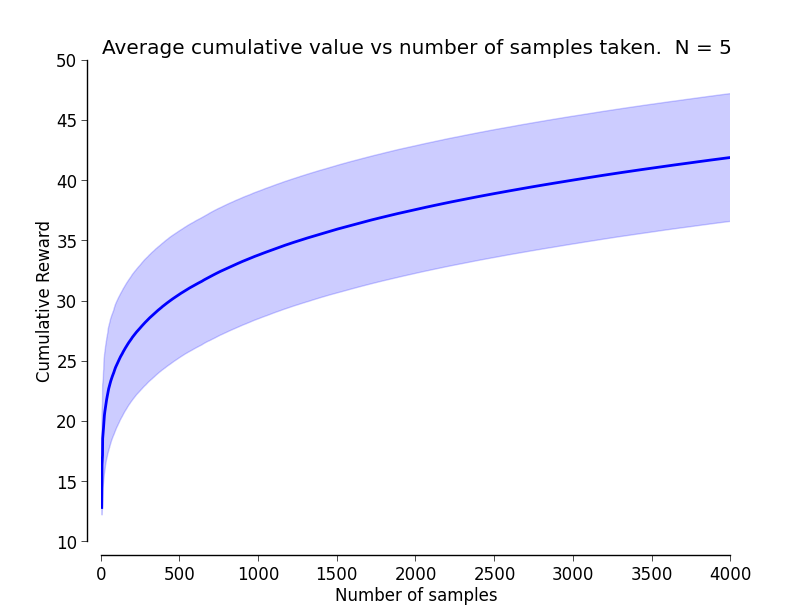
\includegraphics[width=0.8\textwidth]{images/cumulative-reward.png}
	\caption{The reward function plotted is the cumulative reward for sampling from a Gaussian distribution with mean 0 and variance 1.  The cumulative reward is averaged over five trials of 4000 samples.  As the number of samples from a distribution is increased the amount of information gained is reduced.  The reward at any point in time can be viewed as the reduction in Shannon surprise of an instantiation of the random variable as a result of incorporating that value into the learned distribution.  It is important to note that the returns of this reward function decrease with the time spent sampling a particular random variable.  The diminishing returns are necessary to use the Marginal Value Theorem formulation from Charnov \cite{charnov1973optimal}.}
	\label{fig:reward}
\end{figure}

	- Combining foraging models with bandit literature 
		- The previous work on foraging assumed an inherent value to
			options that the agent cared about.  Specifically, energy stored up.
		- We use a valuation model taken from bandit literature.  
		- We use the reward function from Koch's attention models
		- We use the decision making process from foraging. 
		- We add the concept of multi-arrival rate things, awareness of time limits.
	- Previous work had a limit on the number of samples it could take
		- We realized that the actual quantity that limits the exploration process
			is time.
		- By limiting the time and (in this case) relaxing the limit on sample sizes we more accurately deal with productivity.  
	- This experiment models a type of prospecting where the number of samples isn't limited but they do take time. 
	- To that end we are looking at productivity.

	-  This experiment is more akin to contextual bandits.  
	- The image represents a context, the NIRVSS 
	- Apply texturecam classification of a scene, as the context
	- the choice is to sample or continue

	- Productivity 




\section{Section in Appendix}
\label{appendix-sec1}

	Sample text. Sample text. Sample text. Sample text. Sample text. Sample text. 
	Sample text. Sample text. Sample text. Sample text. Sample text. Sample text. 
	Sample text. 

%% References
%%
%% Following citation commands can be used in the body text:
%% Usage of \cite is as follows:
%%   \cite{key}         ==>>  [#]
%%   \cite[chap. 2]{key} ==>> [#, chap. 2]
%%

%% References with bibTeX database:

\bibliographystyle{elsarticle-num}


\bibliography{merged}


\end{document}

%%
%% End of file `elsarticle-template-num.tex'.

